\documentclass[11pt]{scrartcl}
\usepackage[top=2cm, bottom=4.5cm, left=2.5cm, right=2.5cm]{geometry}
\usepackage{graphicx,float}
\usepackage{url}
\usepackage[T1]{fontenc}
\usepackage[font=small,labelfont=bf,tableposition=top]{caption}
%opening
\title{Project Report 1}
\author{Dingyi Zhuang, Tianyu Shi, Fuyuan Lyu}

\begin{document}

\maketitle

\begin{abstract}
This is the abstract.
\end{abstract}

\section{Introduction}

\section{Datasets}
We use four datasets including Ionosphere Dataset\footnote{\url{https://archive.ics.uci.edu/ml/datasets/ionosphere}}, Adult Dataset\footnote{\url{https://archive.ics.uci.edu/ml/datasets/Adult}}, Iris Dataset\footnote{\url{https://archive.ics.uci.edu/ml/datasets/Iris}} and Car Evaluation Dataset\footnote{\url{https://archive.ics.uci.edu/ml/datasets/Car+Evaluation}}. The targets of all these four datasets are categorical classification (including binary classification). We exam four datasets to find that no missing values exist. We use \textit{replace} function in \textit{pandas} module to process all the target values into categorical count value. We will briefly describe the specific features and then introduce how to extract/process the features.

\subsubsection*{Ionosphere Dataset}
Ionosphere dataset contains 34 radar data (real values between -1 and 1)\cite{sigillito1989classification}. We find their distribution with respect to the "good" or "bad" target, which is reflected in Figure \ref{iono_feat}. We then remove radar 1 feature which is always 0. We can see that good class and bad class have quite distinct patterns in the antennas power value, which is essential in the following classification. We also fill between the intervals of good-class feature distribution to find that such surface is quite similar to the auto-correlated signals. Therefore, we use Principal Component Analysis to reduce the dimensions from 34 into 10 to learn the low-rank representation for more efficient and powerful training.

\begin{figure}[t]
	\centering
	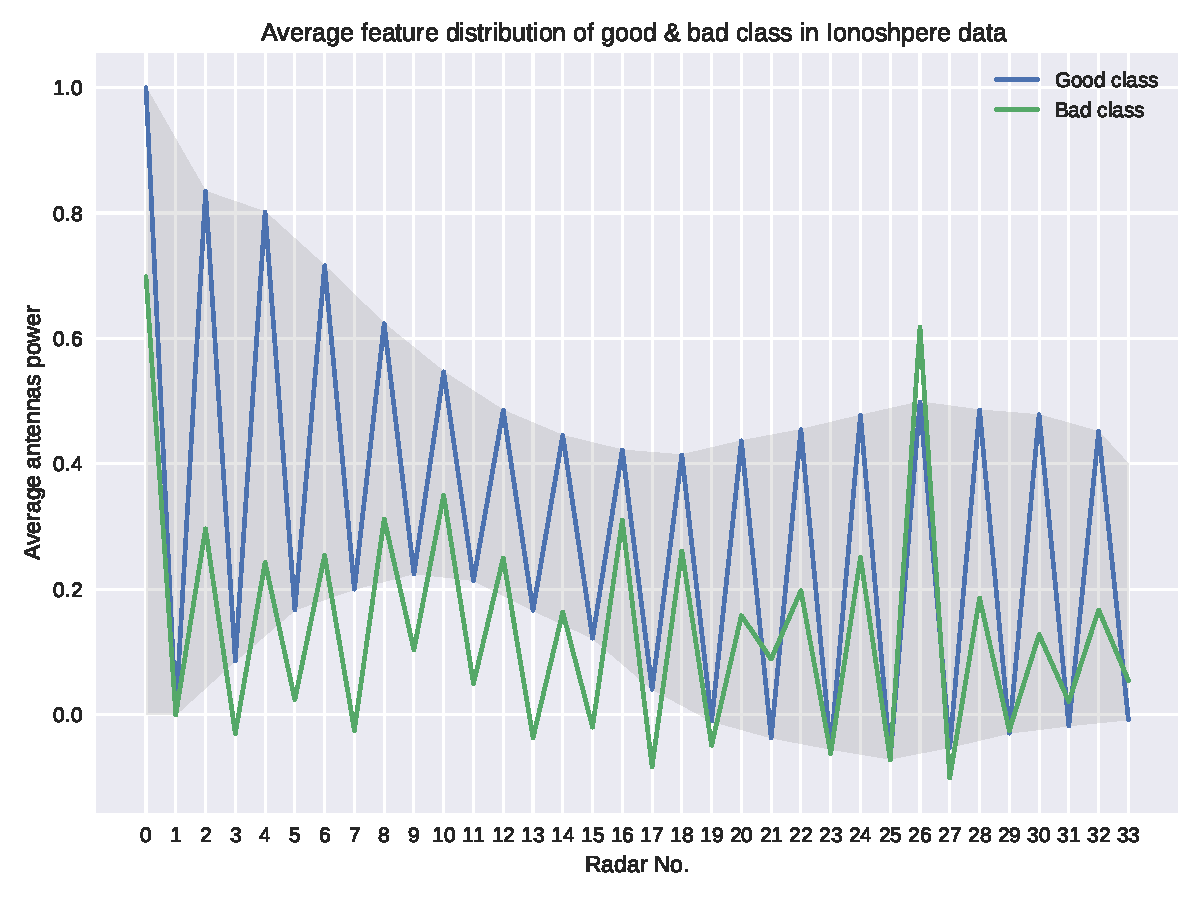
\includegraphics[width=0.8\linewidth]{fig/iono_feat_dist.pdf}
	\caption{Distribution of average numerical features given "good" or "bad" class in ionosphere dataset}
	\label{iono_feat}
\end{figure}

\subsubsection*{Adult Dataset}
Adult dataset aims to predict whether income exceeds \$50K/yr based on census data. There are 14 features included with datatypes of continuous count values, continuous real values and categorical/binary values. We min-max normalize the continuous values (both count and real),  discretize normalized real values into 10 categories and leave everything else untouched.


\subsubsection*{Iris Dataset}
There are continuous real value attributes with 1 decimal precision, whose basic statistic information is listed in Figure \ref{iris_des} and Table \ref{iris_table}, where \textit{sl,sw,pw,pw} stand for \textit{sepal length, sepal width, petal width, petal length}. Linear correlation between features can be found, e.g. petal length \& petal width and petal length \& sepal length. We also min-max normalize and discretize the normed real values.

\begin{figure}[H]
	\begin{minipage}{0.9\linewidth}
		\begin{minipage}[b]{0.5\linewidth}
		  \centering
		  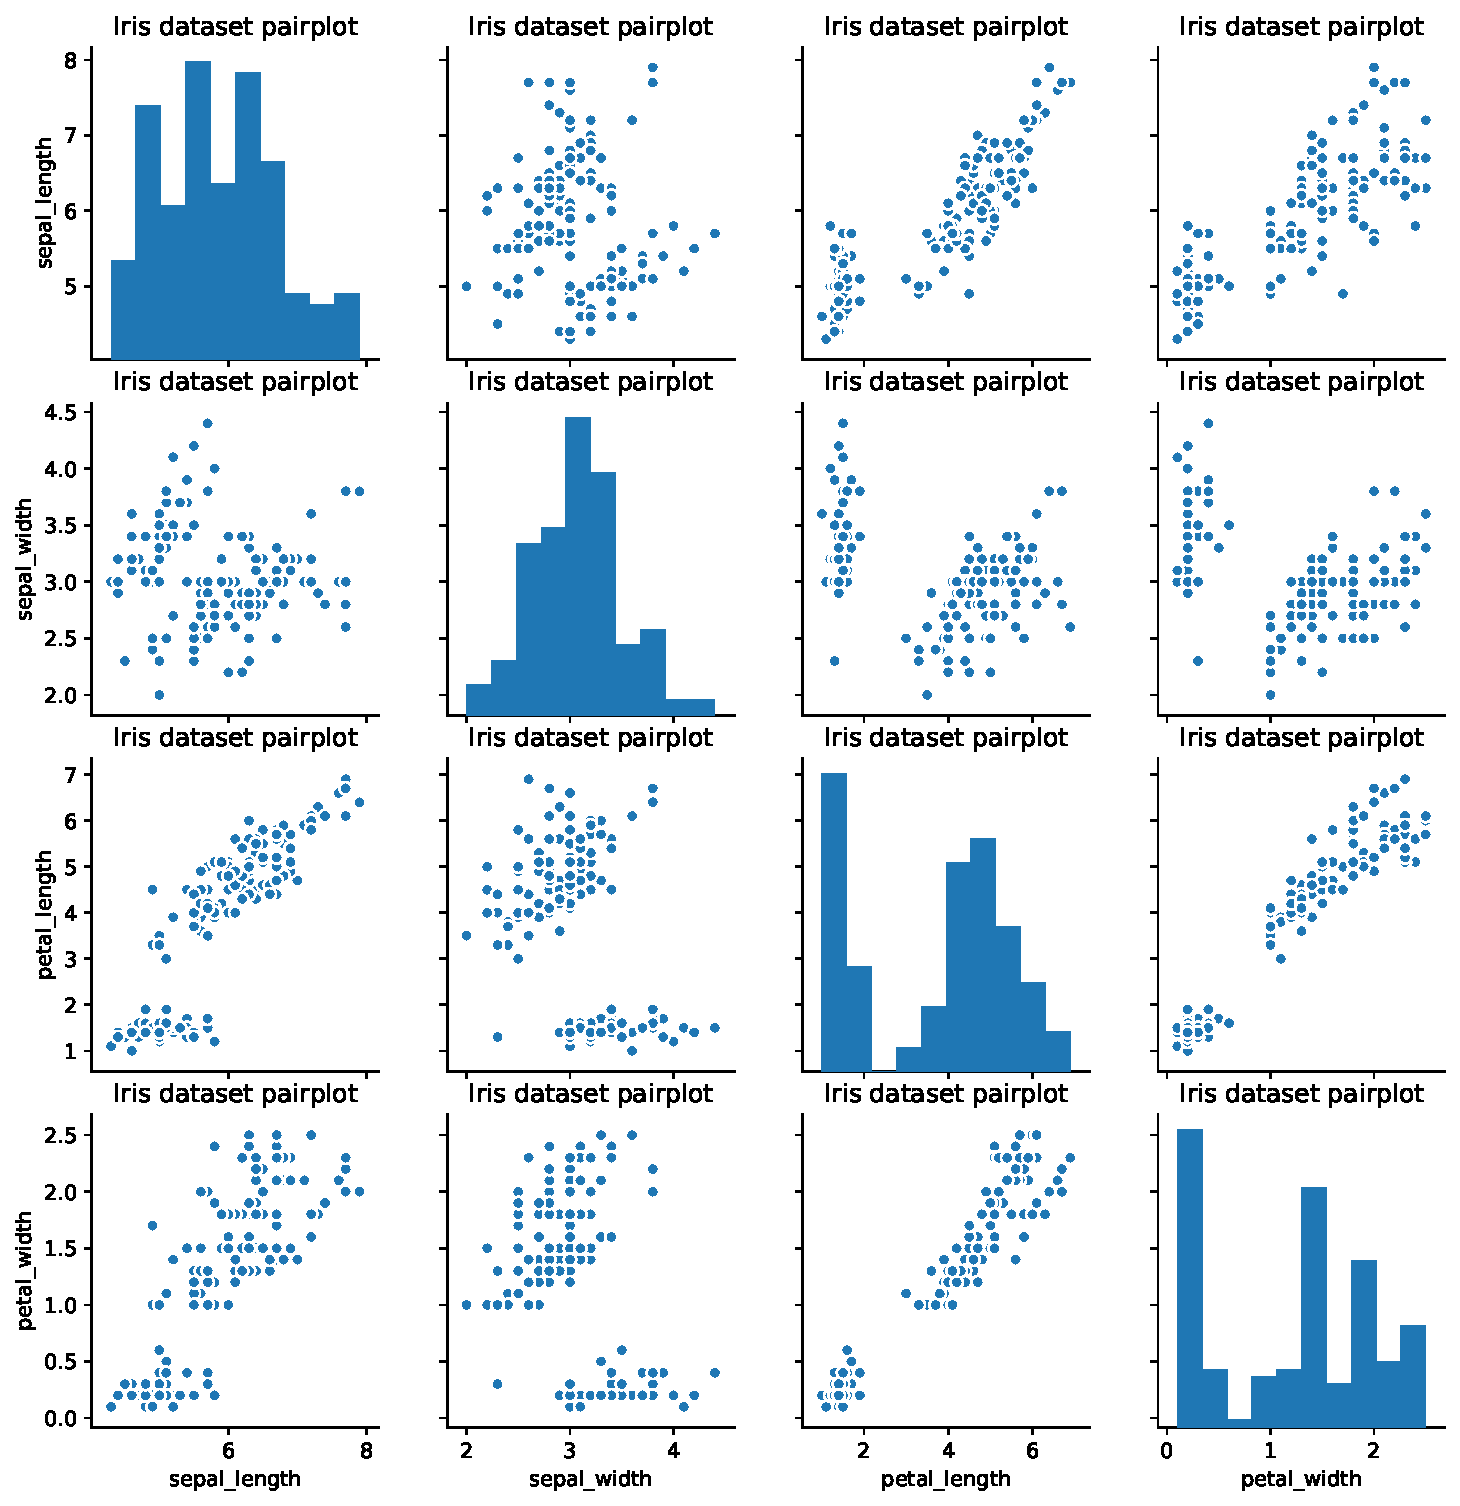
\includegraphics[width= \linewidth]{fig/iris_pairplot.pdf}
		  \captionof{figure}{Pairplot of iris data features}
		  \label{iris_des}
		\end{minipage}
		\hfill
		\begin{minipage}[b]{0.4\linewidth}
		  \centering
			\begin{tabular}{c|cccc}
				\hline
				 & sl & sw & pl & pw \\
				\hline
				count & 150 & 150 & 150 & 150\\
				mean & 5.84 & 3.05 & 3.75 & 1.19\\
				std & 0.82 & 0.43 & 1.76 & 0.76\\
				min & 4.3 & 2.0 & 1.0 & 0.1 \\
				25\% & 5.1 & 2.8 & 1.6 & 0.3\\
				50\% & 5.8 & 3.0 & 4.3 & 1.3\\
				75\% & 6.4 & 3.3 & 5.1 & 1.8 \\
				max & 7.9 & 4.4  & 6.9 & 2.5 \\
				\hline
			\end{tabular} 
		\captionof{table}{Iris data description}
		\label{iris_table}
		\end{minipage}
	\end{minipage}
\end{figure}


\subsubsection*{Car Evaluation Dataset}
In Car Evaluation Dataset, we use some categorical features of cars, e.g. price, door number and capacity, to predict the safety level of the cars. This dataset is quite straightforward, we only transform the raw data into categorical features to predict the categorical safety level.


\section{Results}

\section{Discussion and Conclusion}

\section{Statement of Contributions}

\begin{itemize}
	\item Dingyi Zhunag
	\item Tianyu Shi
	\item Fuyuan Lyu
\end{itemize}

\bibliographystyle{unsrt}
\bibliography{a1}

\end{document}
